\documentclass{article}
\usepackage[utf8]{inputenc}
\usepackage{amsmath}
\usepackage{graphicx}
\usepackage{hyperref}
\usepackage{multicol}
\usepackage{tablefootnote}
\usepackage{float}  % Add this in your preamble
\usepackage{siunitx} % Load the siunitx package
\usepackage{caption}
\usepackage[left=0.7in,right=0.7in,top=1in,bottom=1in]{geometry} % Set margins
\title{A Hybrid Approach to Quantum Circuit Analysis: Leveraging Machine Learning for Error Rate Prediction}

\author{
Hoang Nguyen$^1$ \\
{\small $^1$\textit{Department of Physics, Université de Bourgogne, Dijon, France}}
}


\date{\today}

\begin{document}

\maketitle

\renewcommand{\thefootnote}{\arabic{footnote}}
\setcounter{footnote}{0}

\footnotetext[1]{Long-Hoang\_Nguyen@etu.u-bourgogne.fr}

\begin{abstract}
        This paper introduces a methodology that integrates quantum computing with machine learning to examine a parameterized quantum circuit with three qubits. Initiated by a Hadamard gate, the circuit progresses through RX, RZ, and RY gates, modulated by parameters $\theta$, $\phi$, and $\zeta$, and is linked by controlled-NOT gates, culminating in a measurement phase. The study leverages a dataset of various parameter configurations and corresponding output states to analyze the quantum circuit's error rates using a machine learning model. This model, composed of multiple dense layers, aims to minimize mean squared error loss. The model is trained over 200 epochs to predict error rates based on the input parameters ($\theta$, $\phi$, $\zeta$). Training progress is monitored through plots that demonstrate the model's learning curve. To validate the model's predictive capabilities, actual error rates are compared against model predictions, showing a high degree of accuracy.
\end{abstract}

\begin{multicols}{2}
\section{Introduction}
Introduce the topic of your paper, providing background information and stating the problem you intend to solve or the hypothesis you intend to test. Outline the main contributions of your paper.

\section{Quantum Circuits}

The quantum circuit employed in this study is composed of three qubits initialized in the state $|0\rangle$. The circuit begins with a Hadamard gate applied to the first qubit, creating a superposition state. This is followed by a series of rotation gates—RX, RZ, and RY—acting on the second and third qubits. These rotation gates are parameterized by $\theta$, $\phi$, and $\zeta$, respectively, allowing for a versatile manipulation of the qubit states.
To entangle the qubits and create correlations between them, controlled-NOT (CNOT) gates are employed. The first CNOT gate is applied between the first and second qubits, while the second CNOT gate links the second and third qubits. This sequence of gates aims to generate a complex multi-qubit state that is sensitive to the chosen parameters.
Measurement operations are applied to all qubits at the end of the circuit, collapsing the quantum state into a classical outcome. The resulting state probabilities are determined by the initial parameter settings, making this circuit a suitable testbed for exploring the relationship between parameter choices and resulting quantum states.

\begin{figure}[H]
    \centering
    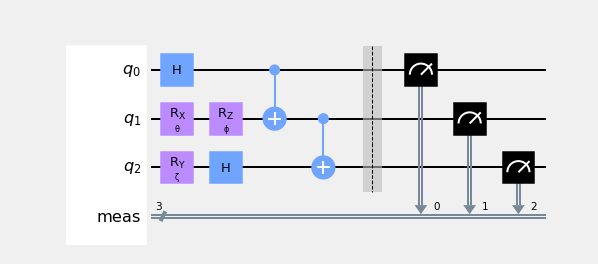
\includegraphics[width=0.45\textwidth]{../quantum_circuit.png}
    \caption{Quantum Circuit}
    \label{fig:quantum_circuit}
\end{figure}

\subsection{Quantum Circuit Simulation}

After constructing the quantum circuit, we simulate it by creating a range of values for each parameter. These parameters, theta ($\theta$), phi ($\phi$), and zeta ($\zeta$), are pivotal for controlling the rotation gates within the quantum circuit. This simulation helps in understanding how various parameter configurations affect the quantum state.

\begin{figure}[H]
        \hspace*{-3.5cm}  % Adjust the value as needed
        \centering
        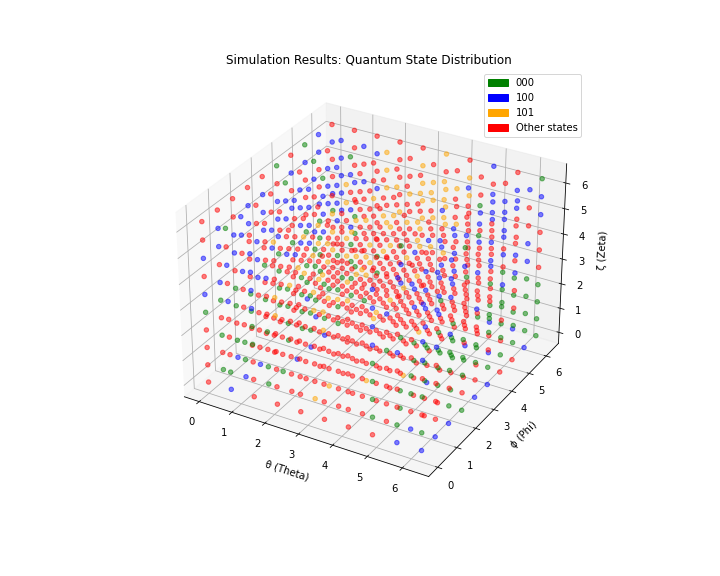
\includegraphics[width=0.80\textwidth]{../3d_simulation_results_plot.png}
        \caption{Quantum Circuit Simulation Results}
        \label{fig:quantum_circuit_simulation}
\end{figure}

\begin{itemize}
    \item \textbf{Parameter Initialization:} The script initializes three parameters: $\theta$, $\phi$, and $\zeta$. These parameters are integral to the rotation gates in the quantum circuit, dictating their respective rotations.
    
    \item \textbf{Circuit Simulation:} A loop is established over a range of values for each parameter. The circuit is simulated for every combination of these values. During each iteration, the circuit parameters are bound to specific values, transpiled for the simulator, and executed.
    
    \item \textbf{Result Collection:} For each set of parameters, the simulation results are collected. These results comprise the counts of measurement outcomes, which reflect the quantum system's state under the influence of the given parameters.
    
    \item \textbf{Visualization:} The results are visualized using a 3D scatter plot. The plot's axes represent the values of $\theta$, $\phi$, and $\zeta$, with each point's color corresponding to the most frequent outcome in the simulation. This visualization provides an intuitive understanding of the quantum system's behavior across different parameter settings.
    
    \item \textbf{Data Export:} The simulation data is formatted and saved into a JSON file for ease of access, further analysis, or sharing with other researchers.
\end{itemize}

The simulation and visualization process elucidates the influence of parameter variations on the quantum system's dynamics, offering a deeper insight into the manipulation of quantum states.

\section{Mathematical Background}
Delve into the mathematical foundation of quantum circuits. Discuss quantum bits (qubits), quantum gates, and their representation in mathematical terms. Cover the mathematical principles that govern the operations of the Hadamard gate (H), the Pauli-X (RX), the Pauli-Z (RZ), the Pauli-Y (RY) gates, and the CNOT gate (CX). Explain how these gates transform the state of qubits and the mathematical representation of these transformations.

\begin{itemize}
        \item \textbf{Hadamard (H) Gate:} Creates a superposition state from a basis state.
        \[
        H = \frac{1}{\sqrt{2}}
        \begin{pmatrix}
            1 & 1 \\
            1 & -1
        \end{pmatrix}
        \]
        
        \item \textbf{RX (Rotation around X-axis) Gate:} Rotates a qubit state around the X-axis of the Bloch sphere by an angle $\theta$.
        \[
        RX(\theta) = 
        \begin{pmatrix}
            \cos\left(\frac{\theta}{2}\right) & -i\sin\left(\frac{\theta}{2}\right) \\
            -i\sin\left(\frac{\theta}{2}\right) & \cos\left(\frac{\theta}{2}\right)
        \end{pmatrix}
        \]
        
        \item \textbf{RY (Rotation around Y-axis) Gate:} Rotates a qubit state around the Y-axis by an angle $\zeta$.
        \[
        RY(\zeta) = 
        \begin{pmatrix}
            \cos\left(\frac{\zeta}{2}\right) & -\sin\left(\frac{\zeta}{2}\right) \\
            \sin\left(\frac{\zeta}{2}\right) & \cos\left(\frac{\zeta}{2}\right)
        \end{pmatrix}
        \]
        
        \item \textbf{RZ (Rotation around Z-axis) Gate:} Rotates a qubit state around the Z-axis by an angle $\phi$.
        \[
        RZ(\phi) = 
        \begin{pmatrix}
            e^{-i\frac{\phi}{2}} & 0 \\
            0 & e^{i\frac{\phi}{2}}
        \end{pmatrix}
        \]
        
        \item \textbf{CNOT (Controlled-NOT) Gate:} An entangling gate that flips the target qubit if the control qubit is in state $|1\rangle$.
        \[
        CNOT = 
        \begin{pmatrix}
            1 & 0 & 0 & 0 \\
            0 & 1 & 0 & 0 \\
            0 & 0 & 0 & 1 \\
            0 & 0 & 1 & 0
        \end{pmatrix}
        \]
    \end{itemize}


\section{Machine Learning Methodology}

    This section delineates the machine learning methodology employed to analyze and predict error rates of the quantum circuit outcomes based on parameter variations. Our approach involves constructing a neural network model capable of fitting a complex, non-linear function to the relationship between the quantum circuit parameters \((\theta, \phi, \zeta)\) and the observed error rates.
    
\subsection{Data Preparation}
    
    The dataset comprises simulation results from various parameter configurations of the quantum circuit. Each data point corresponds to a specific set of parameters and the resultant error rate, calculated by comparing the observed output state to the expected outcome. The error rate serves as an indicator of how the parameter values influence the circuit's performance.
    
\subsection{Model Architecture}
    
    The core of our machine learning approach is a deep neural network with a sequential architecture, consisting of multiple dense layers. Each dense layer is equipped with ReLU activation functions, allowing the model to capture non-linear relationships in the data. The network's depth, with alternating layers, facilitates the learning of intricate patterns in the parameter-error rate mapping.
    
\subsection{Training and Validation}
    
    The model is trained using a dataset split into training and testing sets, ensuring an unbiased evaluation of its predictive capabilities. We employ the mean squared error loss function, which quantifies the discrepancy between the predicted and actual error rates. To optimize the network's weights, we utilize the Nadam optimizer, a variant of the stochastic gradient descent algorithm known for its efficiency in converging to the solution.
    
\subsection{Results and Evaluation}
    
    Upon completion of the training process, which extends over 200 epochs, the model's performance is assessed using the test dataset. Loss curves, plotted against the number of epochs, exhibit the model's learning progression, revealing a steady decrease in both training and validation loss, indicative of effective learning.
    
    The model's predictive accuracy is further substantiated by comparing its predictions against actual error rates. This comparison demonstrates a high level of concordance, thereby validating the model's utility in predicting the quantum circuit's error rates based on the parameter values. 

\subsection{Conclusion}

    The integration of machine learning with quantum circuit analysis has proven effective. The constructed neural network model exhibits a robust predictive capability, making it a valuable tool for understanding and optimizing quantum circuits.
    
\vspace{-1.70cm}  % Adjust the value as needed to move the figure up
\begin{figure}[H]
        \centering
        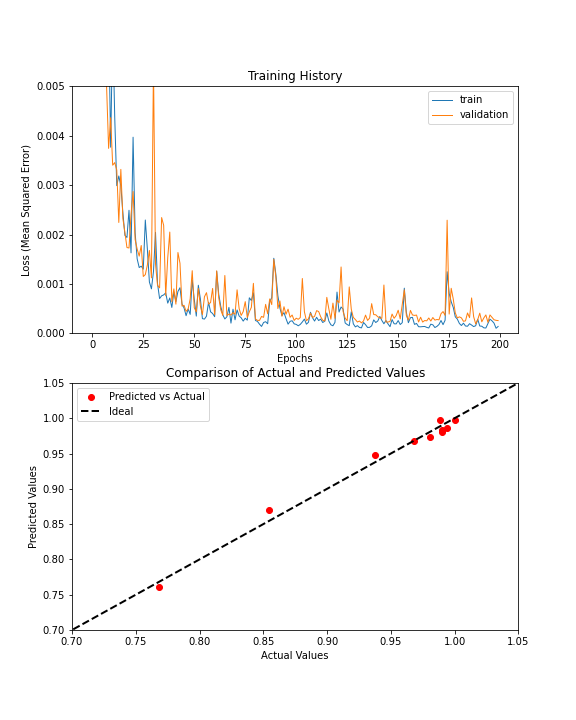
\includegraphics[width=0.55\textwidth]{../combined_plots.png}
        \captionsetup{skip=5pt}  % Adjust the value as needed to move the caption closer
        \caption{Model Loss Over Epochs}
        \label{fig: Model Loss Over Epochs}
\end{figure}
    
    



\section{Methodology}
Detail your experimental setup, the data you've used, and the procedures you've followed.

\section{Results}
\begin{table}[H]
        \centering
        \begin{tabular}{|S[table-format=1.5]|S[table-format=1.5]|}
            \hline
            {Actual Value} & {Predicted Value} \\
            \hline
            0.99023 & 0.98660 \\
            0.99805 & 1.00537 \\
            0.85156 & 0.84636 \\
            0.93262 & 0.93636 \\
            0.99219 & 0.99268 \\
            0.97852 & 0.98278 \\
            0.99316 & 0.99455 \\
            0.98535 & 0.98286 \\
            0.76660 & 0.80205 \\
            0.97363 & 0.96529 \\
            \hline
        \end{tabular}
        \caption{Comparison of Actual and Predicted Values}
        \label{tab:actual_vs_predicted}
\end{table}

\section{Discussion}
Interpret your results, discussing their implications and how they relate to the hypotheses or problems stated in the introduction.


\section{Conclusion}
Summarize your findings, their significance, and potential future work.

\section{References}

\section*{Acknowledgments}
Acknowledge any assistance you received, including funding, advice, and technical help.


\end{multicols}

\end{document}
